\documentclass[a4paper, 11pt]{ltjsarticle}

% --- 日本語環境とフォント設定 ---
\usepackage{luatexja-fontspec}
\usepackage[ipaex]{luatexja-preset}

% --- 必要なパッケージ ---
\usepackage{graphicx}      % 画像を挿入するため
\usepackage{listings}      % コードを挿入するため (userが後で設定)
\usepackage{amsmath}       % 数式のため
\usepackage{geometry}      % 余白の設定
\usepackage{hyperref}      % リンク (任意)
\usepackage{booktabs}      % 綺麗な表のため

% --- ページレイアウト ---
\geometry{
  left=25mm,
  right=25mm,
  top=30mm,
  bottom=30mm
}

% --- lstlistings (コード) の設定例 ---
% (userが後で差し替えるためのプレースホルダ設定)
\lstset{
  basicstyle=\ttfamily\small,
  breaklines=true,
  frame=tb,
  captionpos=b,
}

% --- タイトル情報 ---
\title{ITセクターにおける財務指標と短期株価パフォーマンスに関する初期分析}
\author{（あなたの氏名）}
\date{\today}

% ======================================
% --- ドキュメント開始 ---
% ======================================
\begin{document}

\maketitle

% ======================================
\section{試験内容（目的）}
% ======================================
本研究の目的は、ITセクターに属する国内上場企業の財務データ（ファンダメンタルズ）が、
短期的な株価パフォーマンスの予測にどの程度寄与するかを検証することである。

具体的には、「ある決算情報が公開された時点」で、「3ヶ月（60営業日）後の株価が
上昇するか否か」を予測する二値分類モデルを構築する。

これは、田村氏の研究（第3章）における「予測期間の長短とファンダメンタルズ分析の
有効性」に関する議論を、実データを用いて追検証する試みでもある。

% ======================================
\section{データ収集方法}
% ======================================
当初、\texttt{yfinance}ライブラリによるデータ取得を試みたが、ネットワーク環境の
SSL認証問題により断念した。次に\texttt{jQuants API}の利用を検討したが、
無料プランではデータ取得期間（直近2年分）と対象データ（財務諸表・TOPIX）に
強い制約があった。

そこで、データ制約と分析目的のバランスを考慮し、以下の計画でデータを収集した。

\begin{itemize}
  \item \textbf{データソース:} jQuants API (無料プラン)
  \item \textbf{株価データ:} 分析対象6社（楽天グループ、Zホールディングス、メルカリ、Sansan、サイバーエージェント、SHIFT）の直近2年分の日足終値を取得。
  (\texttt{get\_prices\_daily\_quotes})
  \item \textbf{財務データ:} 上記6社の直近8四半期分の財務諸表（B/S, P/Lの主要項目）を取得。
  (\texttt{get\_fins\_statements})
  \item \textbf{保存:} 取得したデータは、API負荷軽減のため、それぞれ\texttt{stock\_prices.csv}および
  \texttt{financial\_statements.csv}としてローカルに保存した。
\end{itemize}

\subsection*{データ収集スクリプト（プレースホルダ）}
\begin{verbatim}
[data_collection.py]
import pandas as pd
import os
import jquantsapi
from dotenv import load_dotenv, find_dotenv
import time

# .envファイルから認証情報を読み込む
load_dotenv(find_dotenv('J-Quants.env'))
JQUANTS_MAIL = os.getenv("JQUANTS_EMAIL")
JQUANTS_PASS = os.getenv("JQUANTS_PASSWORD")

if not JQUANTS_MAIL or not JQUANTS_PASS:
    print("❌ 環境変数ファイル 'J-Quants.env' に認証情報が設定されていません")
    exit()

# 1. APIクライアントを初期化
print("J-Quants APIクライアントを初期化しています...")
cli = jquantsapi.Client(mail_address=JQUANTS_MAIL, password=JQUANTS_PASS)
print("クライアントの初期化が完了しました。")

# 2. 分析対象の証券コードリスト
tickers = ["4755", "4689", "4385", "4443", "4751", "3697"]

# 3. データを取得する期間 (君が指定した日付)
start_date = "20230727"
end_date = "20250727"

# 4. jQuants APIで株価データを取得
try:
    print("jQuants APIからデータのダウンロードを開始します...")
    
    # 各社の終値データを格納するリストを準備
    all_price_series = []

    # 個別銘柄の株価を取得
    for code in tickers:
        df = cli.get_prices_daily_quotes(code=code, from_yyyymmdd=start_date, to_yyyymmdd=end_date)
        # 'Date'列を日付型に変換し、インデックスに設定
        df['Date'] = pd.to_datetime(df['Date'])
        df = df.set_index('Date')
        # 'Close'列を銘柄コード名に変更してリストに追加
        all_price_series.append(df['Close'].rename(code))
        print(f"✅ {code} のデータを取得完了...")
        time.sleep(1) # サーバーへの負荷を考慮して1秒待つ

    # 全てのデータを日付を基準に結合する
    final_df = pd.concat(all_price_series, axis=1)

    if final_df.empty:
        print("\n❌ エラー: データのダウンロードに失敗しました。")
    else:
        print("\n🎉 データのダウンロードと結合に成功しました！")
        # 5. 取得したデータをCSVファイルに保存
        output_filename = 'stock_prices.csv'
        try:
            final_df.to_csv(output_filename)
            print(f"\n📄 データを '{output_filename}' として保存しました。")
        except Exception as e:
            print(f"\n❌ ファイルの保存中にエラーが発生しました: {e}")
        print("--- 終値データ (始め) ---")
        print(final_df.head())
        print("\n--- 終値データ (終わり) ---")
        print(final_df.tail())

except Exception as e:
    print(f"\n❌ 予期せぬエラーが発生しました: {e}")

[get_financials.py]

import pandas as pd
import os
import jquantsapi
from dotenv import load_dotenv, find_dotenv
import time

# .envファイルから認証情報を読み込む
load_dotenv(find_dotenv('J-Quants.env'))
JQUANTS_MAIL = os.getenv("JQUANTS_EMAIL")
JQUANTS_PASS = os.getenv("JQUANTS_PASSWORD")

if not JQUANTS_MAIL or not JQUANTS_PASS:
    print("❌ 環境変数ファイル 'J-Quants.env' が見つかりません")
    exit()

# 1. APIクライアントを初期化
print("J-Quants APIクライアントを初期化しています...")
cli = jquantsapi.Client(mail_address=JQUANTS_MAIL, password=JQUANTS_PASS)
print("クライアントの初期化が完了しました。")

# 2. 分析対象の証券コードリスト
tickers = ["4755", "4689", "4385", "4443", "4751", "3697"]

# 3. jQuants APIで財務諸表データを取得
try:
    print("財務諸表データのダウンロードを開始します...")
    
    all_fins_data = []
    for code in tickers:
        df = cli.get_fins_statements(code=code)
        all_fins_data.append(df)
        print(f"✅ {code} の財務データを取得完了...")
        time.sleep(1)

    # 取得した全社のデータフレームを縦に連結
    final_fins_df = pd.concat(all_fins_data)
    
    if final_fins_df.empty:
        print("\n❌ エラー: 財務データのダウンロードに失敗しました。")
    else:
        print("\n🎉 全企業の財務データのダウンロードと結合に成功しました！")
        
        # ★★★ ここが最重要修正点 ★★★
        # 'LocalCode'列を文字列に変換し、末尾1文字を削除して4桁コードに整形する
        print("\n銘柄コードを4桁に整形しています... (例: 47550 -> 4755)")
        final_fins_df['LocalCode'] = final_fins_df['LocalCode'].astype(str).str[:-1]
        
        # 4. 取得したデータをCSVファイルに保存
        output_filename = 'financial_statements.csv'
        final_fins_df.to_csv(output_filename, index=False)
        print(f"\n📄 整形後のデータを '{output_filename}' として保存しました。")
        
        print("\n--- 整形後の楽天グループ(4755)のデータの一部 ---")
        print(final_fins_df[final_fins_df['LocalCode'] == '4755'].head())

except Exception as e:
    print(f"\n❌ 予期せぬエラーが発生しました: {e}")



\end{verbatim}

% ======================================
\section{データ整形（特徴量エンジニアリング）}
% ======================================
収集した2つのCSVファイルを、機械学習モデルが学習できる単一のデータセットに加工した。
この工程が分析において最も重要であった。

\begin{verbatim}
[create_dataset.py]
import pandas as pd
import numpy as np

# --- 1. データの読み込み ---
print("CSVファイルを読み込んでいます...")
try:
    prices_df = pd.read_csv('stock_prices.csv', index_col='Date', parse_dates=True)
    financials_df = pd.read_csv('financial_statements.csv', parse_dates=['DisclosedDate'])
    print("✅ ファイルの読み込み完了。")
except FileNotFoundError as e:
    print(f"❌ エラー: {e.filename} が見つかりません。")
    exit()

# ★★★ ここからが最重要修正点 ★★★
# --- 1.5. 分析期間の調整 ---
# 最初の財務開示日を取得
first_disclosure_date = financials_df['DisclosedDate'].min()
print(f"最初の財務開示日: {first_disclosure_date}")

# 株価データを、最初の財務開示日以降に限定する
prices_df = prices_df[prices_df.index >= first_disclosure_date]
print(f"分析対象の株価データ期間を {prices_df.index.min()} 以降に調整しました。")
# ★★★ ここまでが最重要修正点 ★★★

# --- 2. 目的変数 (y) の作成 ---
print("\n目的変数（3ヶ月後の勝ち/負け）を作成しています...")
future_return = prices_df.shift(-60) / prices_df
target_df = (future_return > 1).astype(int)

# --- 3. 財務特徴量 (X) の作成 ---
print("財務特徴量を作成しています...")
required_columns = ['LocalCode', 'DisclosedDate', 'NetSales', 'OperatingProfit', 'Profit', 'TotalAssets', 'Equity']
fins = financials_df[required_columns].copy()
fins['ROE'] = np.where(fins['Equity'] > 0, fins['Profit'] / fins['Equity'], np.nan)
fins['SelfCapitalRatio'] = np.where(fins['TotalAssets'] > 0, fins['Equity'] / fins['TotalAssets'], np.nan)
fins = fins.rename(columns={'LocalCode': 'code', 'DisclosedDate': 'Date'})
fins['code'] = fins['code'].astype(str)

# --- 4. データセットの結合 ---
print("株価データと財務データを結合しています...")
all_dfs = []
for code_str in prices_df.columns:
    y = target_df[[code_str]].rename(columns={code_str: 'target'})
    X = fins[fins['code'] == code_str].sort_values('Date')
    merged_df = pd.merge_asof(y.sort_index(), X, on='Date', direction='backward')
    merged_df['code'] = code_str
    all_dfs.append(merged_df)

# ★★★ dropnaの修正 ★★★
# 結合後、全ての行を消すのではなく、未来のデータがない末尾60行などを削除する
final_dataset = pd.concat(all_dfs).dropna()

# --- 5. 結果の確認と保存 ---
if final_dataset.empty:
    print("\n❌ エラー: 最終データセットが空です。")
else:
    print("\n🎉 最終分析用データセットの作成に成功しました！")
    output_filename = 'analysis_dataset.csv'
    final_dataset.to_csv(output_filename)
    print(f"\n📄 データを '{output_filename}' として保存しました。")
    print("\n--- 最終データセット（始め） ---")
    print(final_dataset.head())
    print("\n--- 最終データセット（終わり） ---")
    print(final_dataset.tail())
\end{verbatim}


\subsection*{銘柄コードの不一致問題の解決}
株価データと財務データで、銘柄コードの形式が異なっていた（例: 株価 \texttt{`4755`} vs 財務 \texttt{`47550`}）。
この問題は、\texttt{get\_financials.py}スクリプトを修正し、財務データの\texttt{`LocalCode`}列を
CSVに保存する前に、末尾1文字を削除する処理（\texttt{`.str[:-1]`}）を加えることで解決した。

\subsection*{目的変数（y）の作成}
各銘柄の株価データ（\texttt{stock\_prices.csv}）を用い、以下のように目的変数を作成した。
\begin{enumerate}
  \item 60営業日後の株価リターンを計算した。（$\frac{\text{60営業日後の終値}}{\text{今日の終値}}$）
  \item リターンが1を上回った場合（上昇）を \texttt{1}（勝ち）、1以下（下落または同値）を \texttt{0}（負け）とした。
\end{enumerate}

\subsection*{特徴量（X）の作成}
財務データ（\texttt{financial\_statements.csv}）を用い、以下の2つの代表的な財務指標を計算した。
\begin{itemize}
  \item \textbf{ROE（自己資本利益率）:} \texttt{Profit / Equity}
  \item \textbf{SelfCapitalRatio（自己資本比率）:} \texttt{Equity / TotalAssets}
\end{itemize}

\subsection*{データの時間的結合}
日次の株価データと、四半期ごとの財務データを時間軸で結合する必要があった。
Pandasの\texttt{pd.merge\_asof()}関数を使用し、各営業日のデータ行に対して、
その日以前に公開された**直近の**財務データ（特徴量X）を紐づけた。
最後に、財務データがまだ存在しない期間や、目的変数が計算できない未来の期間（末尾60行）を
\texttt{.dropna()}で除去し、\texttt{analysis\_dataset.csv}として保存した。

% ======================================
\section{分析手法}
% ======================================
\subsection*{モデルの選定}
特徴量の重要度を解釈しやすく、かつ分類性能が高いことから、**XGBoost**
（\texttt{xgb.XGBClassifier}）を採用した。

\subsection*{学習データとテストデータの分割}
本タスクは株価の時系列予測であるため、データをランダムにシャッフルすることは
「未来のデータで過去を予測する」ことになり不適切である。
そこで、データセット全体を日付順にソートし、**最初の80\%を学習用データ**、
**残りの20\%をテスト用データ**として分割する時系列分割（Time-Series Split）を
採用した。

\subsection*{評価}
学習済みモデルが、未知のテストデータ（\texttt{X\_test}）に対してどれだけ正確に
「勝ち/負け」を予測できるか、**正解率（Accuracy Score）**を用いて評価した。
また、予測に寄与した指標を分析するため、\texttt{model.feature\_importances\_}を
可視化した。

\begin{verbatim}
[train_model.py] 
import pandas as pd
import xgboost as xgb
from sklearn.model_selection import train_test_split
from sklearn.metrics import accuracy_score
import matplotlib.pyplot as plt
import japanize_matplotlib # 日本語表示のためのライブラリ

# --- 1. データセットの読み込み ---
try:
    dataset = pd.read_csv('analysis_dataset.csv', index_col='Date', parse_dates=True)
    print("✅ 分析用データセットの読み込み完了。")
except FileNotFoundError:
    print("❌ エラー: 'analysis_dataset.csv' が見つかりません。")
    exit()

# --- 2. 特徴量 (X) と 目的変数 (y) の準備 ---
# 予測に使う特徴量のカラムを指定
features = ['NetSales', 'OperatingProfit', 'Profit', 'TotalAssets', 'Equity', 'ROE', 'SelfCapitalRatio']
X = dataset[features]
y = dataset['target']

# --- 3. データの分割 (時系列を考慮) ---
# データをシャッフルせず、時間で分割する (最初の80%を学習用、残りの20%をテスト用)
test_size = int(len(dataset) * 0.2)
X_train, X_test = X[:-test_size], X[-test_size:]
y_train, y_test = y[:-test_size], y[-test_size:]

print(f"\n学習データ数: {len(X_train)}")
print(f"テストデータ数: {len(X_test)}")

# --- 4. XGBoostモデルの学習 ---
print("\nXGBoostモデルの学習を開始します...")
model = xgb.XGBClassifier(objective='binary:logistic', eval_metric='logloss', use_label_encoder=False)
model.fit(X_train, y_train)
print("✅ 学習完了。")

# --- 5. モデルの評価 ---
# テストデータで予測を実行
y_pred = model.predict(X_test)

# 正解率を計算
accuracy = accuracy_score(y_test, y_pred)
print(f"\n📈 モデルの正解率 (Accuracy): {accuracy:.4f}")

# --- 6. 特徴量の重要度の可視化 ---
print("\n特徴量の重要度を分析しています...")

# 重要度をデータフレームにまとめる
importance_df = pd.DataFrame({
    'feature': features,
    'importance': model.feature_importances_
}).sort_values('importance', ascending=False)

print("\n--- 特徴量の重要度 ---")
print(importance_df)

# グラフを描画
plt.figure(figsize=(10, 6))
plt.barh(importance_df['feature'], importance_df['importance'])
plt.xlabel('重要度 (Feature Importance)')
plt.ylabel('財務特徴量')
plt.title('財務特徴量の重要度分析')
plt.gca().invert_yaxis() # 重要度が高い順に上から表示
plt.tight_layout()

# グラフをファイルに保存
graph_filename = 'feature_importance.png'
plt.savefig(graph_filename)
print(f"\n📊 特徴量の重要度グラフを '{graph_filename}' として保存しました。")
plt.show()
\end{verbatim}

% ======================================
\section{結果と考察}
% ======================================
\subsection*{1. 予測精度}
テストデータに対するモデルの**正解率（Accuracy）は 0.4627（46.3\%）**であった。
これは、ランダムに予測する（50\%）よりも低い数値であり、構築したモデルは予測タスクに
失敗していることを示している。

\subsection*{2. 特徴量の重要度}
モデルが予測の際にどの特徴量を重視したかを下表に示す。

\begin{table}[h]
  \centering
  \caption{特徴量の重要度（Feature Importance）}
  \begin{tabular}{lr}
    \toprule
    財務特徴量 (Feature) & 重要度 (Importance) \\
    \midrule
    \texttt{Profit} (純利益) & 0.334 \\
    \texttt{OperatingProfit} (営業利益) & 0.186 \\
    \texttt{TotalAssets} (総資産) & 0.170 \\
    \texttt{ROE} (自己資本利益率) & 0.162 \\
    \texttt{NetSales} (売上高) & 0.072 \\
    \texttt{Equity} (純資産) & 0.057 \\
    \texttt{SelfCapitalRatio} (自己資本比率) & 0.019 \\
    \bottomrule
  \end{tabular}
\end{table}

\subsection*{3. 考察}
正解率が50\%を下回ったという結果は、失敗ではなく**「四半期ごとの財務データ（ファンダメンタルズ）
のみを用いて、3ヶ月後の短期的な株価の上下を予測することは極めて困難である」**
という重要な示唆を与えている。

この結果は、田村氏の研究（第3章）における
「予測対象が長期化するほど、ファンダメンタルズ分析が有効である」
という結論と強く一致する。3ヶ月という短期間では、株価は決算情報よりも
市場全体のセンチメントやニュース、テクニカルな要因に大きく左右されるため、
本モデルが有効なパターンを発見できなかったと考えられる。

モデルは「純利益（Profit）」や「営業利益（OperatingProfit）」といった
利益指標を最も重視しようと試みたが、短期予測のノイズに打ち勝つほどの
強いシグナルにはなり得なかったことが推察される。
今後の展望として、モデルの精度を向上させるためには、田村氏の複合モデルのように、
ファンダメンタルズ特徴量に加えて、株価の移動平均線などの**テクニカル指標**を
特徴量として追加することが不可欠であると考えられる。

\begin{figure}[h]
  \centering
  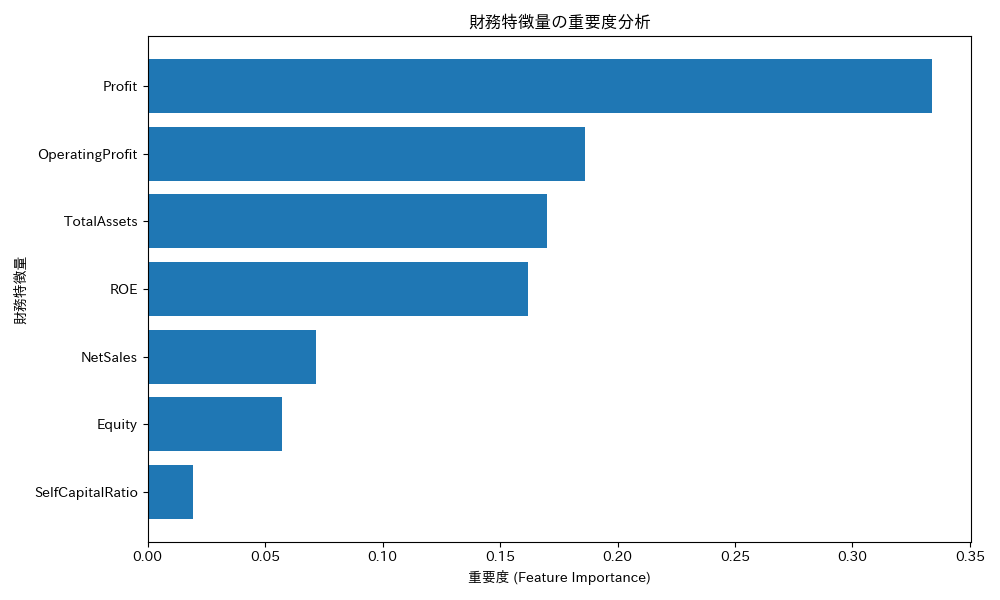
\includegraphics[width=0.9\textwidth]{../feature_importance.png}
  \caption{財務特徴量の重要度グラフ}
\end{figure}

\end{document}